\documentclass{beamer}
\usepackage{beamerthemeOerestad}
\usetheme{Oerestad}

\usepackage[utf8]{inputenc}
\usepackage{amsfonts}
\usepackage{amsmath}
\usepackage{booktabs}
\usepackage{color}
\usepackage{colortbl}
\usepackage{dirtytalk}
\usepackage{graphicx}
\usepackage{hyperref}
\usepackage{listings}
\usepackage[square,sort,comma,numbers]{natbib}
\usepackage{url}
\usepackage{semantic}
\usepackage{tikz}
\usepackage{todonotes}

\hypersetup{
  colorlinks=true,
  urlcolor=cyan
}

\lstdefinestyle{Racket}{
  language=Lisp,
  basicstyle=\ttfamily,
  otherkeywords={\#lang,define,match,let,:,->,lambda,struct,define-type,car,cdr},
  identifierstyle=\color{pink!60!blue},
  keywordstyle=\color{blue!50!black},
  stringstyle=\color{green!50!black},
  commentstyle=\color{pink!60!black}
}

\lstdefinestyle{Java}{
  language=Java,
  basicstyle=\ttfamily
}

\lstset{
  style=Racket
}

\usetikzlibrary{shapes.multipart, chains, positioning}
\tikzset{cons/.style n args=2{
    on chain,
    rectangle split,
    rectangle split horizontal,
    rectangle split parts=2,
    draw,
    anchor=center,
    text height=1.5ex,
    node contents={#1\nodepart{two}#2},
    join={by ->}
  }
}

\title{Functional Programming in Typed Racket}
\author{Florian Biermann \\\small{\texttt{fbie@itu.dk}} \\~}

\institute{IT University of Copenhagen \& UCAS}

\date{2016-05-26}

\begin{document}

\begin{frame}
  \titlepage{}
\end{frame}

\begin{frame}{Who am I?}
  Just call me Florian!

  \begin{itemize}
  \pause{} \item I am from Germany and live in Denmark.
  \pause{} \item Second year PhD student at IT University of Copenhagen and UCAS.
  \pause{} \item My Chinese is really bad (but I am trying to learn!)
  \pause{} \item If you do not understand what I say or if I speak too fast, \textbf{please tell me right away!}
  \end{itemize}
\end{frame}

\begin{frame}{GitHub Course Page}
  All slides and course materials are available on:

  \begin{center}
    \url{https://github.com/fbie/parallel-functional-lectures}
  \end{center}
\end{frame}

\begin{frame}{Why Functional Programming?}

  Functional programming is old but recently it has become very popular!

  \begin{itemize}
  \pause{} \item Makes it easier to think about what a program does.
  \pause{} \item Parallel in its nature $\rightarrow$ easy to parallelize (next lecture).
  \pause{} \item Used in financial industry, modern compilers and more.
  \pause{} \item Jobs in functional programming pay better!
  \end{itemize}

\end{frame}

\begin{frame}{Typed Racket}

  \begin{center}
    \includegraphics[width=0.2\textwidth]{racket.png}
  \end{center}

  \textbf{Racket} and its sister-language \textbf{Typed Racket} are Scheme-dialects.

  \begin{itemize}
  \pause{} \item Racket is dynamically typed, Typed Racket has a static, strong type system.
  \pause{} \item Functional language, no side-effects (mostly).
  \pause{} \item Good for meta-programming (we won't look at that).
  \end{itemize}
\end{frame}

\begin{frame}[fragile]{Hello World in Typed Racket}
\begin{center}
\begin{lstlisting}
;; This is a comment!
;; Tell the run-time, which language to use.
#lang typed/racket

;; Now, print something.
(print "Nihao!")
\end{lstlisting}
\end{center}
\end{frame}

\begin{frame}[fragile]{A More Interesting Program}
\begin{lstlisting}
#lang typed/racket

;; Define x as the result of the computation.
(define x (* (+ 2 4) (+ 42 9)))
\end{lstlisting}

\pause{}

We can check its value in the interactive mode:

\begin{lstlisting}
> x
59
\end{lstlisting}

\end{frame}

\begin{frame}[fragile]{Do You Think This Looks Strange?}

  In Racket, all expressions are written like this:

  \begin{center}
    \lstinline{(function arg1 arg2 ... argN)}
  \end{center}

  \pause{}

  Operators are also just functions:

  \begin{center}
    \begin{tabular}{ccc}
      \lstinline{(+ x y)} & $\Rightarrow$ & $x + y$ \\
      \lstinline{(> x y)} & $\Rightarrow$ & $x > y$ \\
      \lstinline{(/ x y)} & $\Rightarrow$ & $\frac{x}{y}$ \\
      \lstinline{(f x y)} & $\Rightarrow$ & $f(x, \, y)$
    \end{tabular}
  \end{center}

  \pause{}

  Some functions are \textit{variadic}:

  \begin{center}
    \begin{tabular}{ccc}
      \lstinline{(+ x y z)} & $\Rightarrow$ & $x + y + z$
    \end{tabular}
  \end{center}

\end{frame}

\begin{frame}[fragile]{Local Bindings}

Just like local variables in Java, but you can never change them!

\begin{lstlisting}
#lang typed/racket

(let ([x (* 2 16)]
      [y (* 3 17)])
    (print (+ x y)))
\end{lstlisting}

What does this program do?

\vspace{1cm}

\textit{Note:} You cannot reference \lstinline{x} and \lstinline{y} after the last closing parenthesis of the \lstinline{let} expression!

\end{frame}

\begin{frame}[fragile]{The Same Program in Java}
\begin{lstlisting}[style=Java]
public static void main(String[] args) {
  int x = 2 * 16;
  int y = 3 * 17;
  System.out.println(x + y);
}
\end{lstlisting}
\end{frame}

\begin{frame}[fragile]{A First Function}
\begin{lstlisting}
#lang typed/racket

(: times-two (-> Number Number))
(define (times-two x)
  (* 2 x))
\end{lstlisting}

\pause{}

Several new things on this slide:

\begin{itemize}
\pause{} \item Functions need no return statement. Their return value is the last executed statement!
\pause{} \item Type annotations start with \lstinline{:} and describe the type of a symbol.
\pause{} \item The type of \lstinline{times-two} is $Number \, \rightarrow \, Number$.
\end{itemize}
\end{frame}

\begin{frame}[fragile]{Types in Typed Racket}
We write the function type $A \, \rightarrow \, B$ as:

\begin{center}
  \lstinline{(-> A B)}
\end{center}

where \lstinline{A} is the parameter type and \lstinline{B} is the return type.

\vspace{1.5cm}

\pause{}

\begin{center}
  \lstinline{(-> A B C)}
\end{center}

Which types are parameter types, which ones are return types?
\end{frame}

\begin{frame}[fragile]{A Second Function}
\begin{lstlisting}
(: funny (-> Number Number)
(define (funny x)
  (if (< x 0)
      (- x)
      x))
\end{lstlisting}

\vspace{1.5cm}

\pause{}

Conditionals have the form \lstinline{(if B E1 E2)}.
\end{frame}

\begin{frame}[fragile]{Polymorphic Types}
Polymorphic types in Typed Racket are very explicit:

\begin{lstlisting}
(: twice (All (A) (-> A (Pairof A A))))
(define (twice a)
  (cons a a))
\end{lstlisting}

\pause{}

\vspace{0.5cm}

\say{For all types \lstinline{A}, the type of \lstinline{twice} is such that iff you pass it a value of some type \lstinline{A} it will return a pair of type \lstinline{A} $\times$ \lstinline{A}.}

\vspace{1cm}

\pause{}

It's just like generic types in Java!
\end{frame}

\begin{frame}[fragile]{The Same Program in Java}
\begin{lstlisting}[style=Java]
public static Pairof<A, A> twice(A a) {
  return new Pairof<A, A>(a);
}
\end{lstlisting}

\vspace{1.5cm}

\textbf{Note:} There is no build-in pair type in Java :(
\end{frame}

\begin{frame}[fragile]{State is Immutable!}

You cannot change a variable's value. Instead, use \textbf{recursion}:

\begin{lstlisting}
(: is-even? (-> Integer Boolean))
(define (is-even? n)
  (if (< 0 n)
      (is-even? (- n 2))
      (= n 0)))
\end{lstlisting}

\pause{}

Now, we can call the function:

\begin{lstlisting}
> (is-even? 1)
#f
\end{lstlisting}
\pause{}
\begin{lstlisting}
> (is-even? 2048)
#t
\end{lstlisting}
\end{frame}

\begin{frame}[fragile]{The Same Program in Java}
\begin{lstlisting}[style=Java]
public static bool isEven(int n) {
  while (0 < n)
    n = n - 2;
  return n == 0;
}
\end{lstlisting}
\end{frame}

\begin{frame}[fragile]{Anonymous Functions}
You can define functions without giving them a name. Such functions are called \textit{lambda expressions}:

\begin{lstlisting}
> ((lambda (x) x) 2)
2
\end{lstlisting}

\pause{}

Here, we have defined a lambda expression and applied it to the value \lstinline{2}. We call this function  the \textit{identity function}. It is the same as

\begin{center}
$\lambda\, x\, .\, x$
\end{center}

\pause{}

\vspace{.5cm}

We will often come across lambda expressions in functional programming!
\end{frame}

\begin{frame}[fragile]{Structs in Typed Racket}
Structs are containers for values.

\begin{lstlisting}
(struct (myNumberBox
              [v : Number]))

(struct (myNumberStringBox
             ([n : Number] [s : String])))
\end{lstlisting}

\pause{}

We can also use type polymorphism here:

\begin{lstlisting}
(struct (A) (myPolyBox [value : A]))
\end{lstlisting}
\end{frame}

\begin{frame}{That Was a Quick Intro}
  Next, we will do a live coding session!

  \begin{itemize}
  \pause{} \item I code on the big screen and show you how to do functional programming in Racket.
  \pause{} \item You help with ideas and suggestions and experiment yourselves!
  \pause{} \item All code we write will be available on
  \begin{itemize}
  \item \url{github.com/fbie/parallel-functional-programming}
  \end{itemize}
  \pause{} \item You can download Racket from
  \begin{itemize}
  \item \url{racket-lang.org}
  \end{itemize}
  \end{itemize}
\end{frame}

\begin{frame}[fragile]{Java Equivalent to Maybe}
\begin{lstlisting}[style=Java]
public abstract class Maybe<A> {}

public class None<A> extends Maybe<A> {
  public None() {}
}
public class Some<A> extends Maybe<A> {
  public final A a;
  public Some(A a) {
    this.a = a;
  }
}
\end{lstlisting}
\end{frame}

\begin{frame}[fragile]{Singly-Linked Cons List 1/2}
\begin{lstlisting}
(define xs (cons 'a (cons 'b
    (cons 'c (cons 'd (cons 'e '()))))))
\end{lstlisting}

\pause{}

Get the first element of \lstinline{xs}, the ``head'':

\begin{lstlisting}
> (first xs)
'a
> (cdr xs)
'a
\end{lstlisting}

\pause{}

Get the remaining part of \lstinline{xs}, the ``tail'':

\begin{lstlisting}
> (rest xs)
'('b 'c 'd 'e)
> (cdr xs)
'('b 'c 'd 'e)
\end{lstlisting}
\end{frame}

\begin{frame}[fragile]{Singly-Linked Cons List 2/2}
References to tail \textbf{cannot be changed}, because all \textbf{references are immutable}:

\vspace{.5cm}

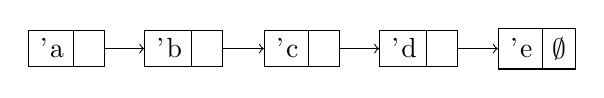
\begin{tikzpicture}[start chain=going right]
  \node (a) [cons={\lstinline{'a}}{}];
  \node (b) [cons={\lstinline{'b}}{}];
  \node (c) [cons={\lstinline{'c}}{}];
  \node (d) [cons={\lstinline{'d}}{}];
  \node (e) [cons={\lstinline{'e}}{$\emptyset$}];
\end{tikzpicture}

\pause{} \vspace{.5cm}

If we want to remove an element, we must build a new list, but we can re-use the tail of the element that we have deleted:

\begin{lstlisting}
(remove xs 'c)
\end{lstlisting}

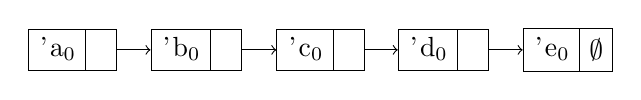
\begin{tikzpicture}[start chain=going right]
  \node (a) [cons={\lstinline{'a}$_0$}{}];
  \node (b) [cons={\lstinline{'b}$_0$}{}];
  \node (c) [cons={\lstinline{'c}$_0$}{}];
  \node (d) [cons={\lstinline{'d}$_0$}{}];
  \node (e) [cons={\lstinline{'e}$_0$}{$\emptyset$}];
\end{tikzpicture}
\pause{}
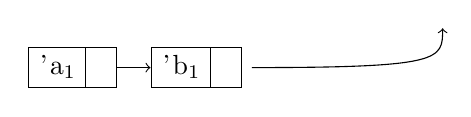
\begin{tikzpicture}[start chain=going right]
  \node (a) [cons={\lstinline{'a}$_1$}{}];
  \node (b) [cons={\lstinline{'b}$_1$}{}];
  \draw [->] (2.277, .0) .. controls (4.7, .0) and (4.7, .1) .. (4.7, .5);
\end{tikzpicture}

\end{frame}

\begin{frame}[fragile]{Java Equivalent to Cons List}
\begin{lstlisting}[style=Java]
public abstract class LinkedList<A> {}

public class Nil<A> extends LinkedList<A> {
  public Nil() {}
}
public class Cons<A> extends LinkedList<A> {
  public final A a;
  public final LinkedList<A> tail;

  public Cons(A a, LinkedList<A> tail) {
    this.a = a;
    this.tail = tail;
  }
}
\end{lstlisting}
\end{frame}

\begin{frame}[fragile]{Java Equivalent to Binary Tree}
\begin{lstlisting}[style=Java]
public abstract class BinaryTree<A> {}

public class Leaf<A> extends BinaryTree<A> {
  public final A a;
  public Leaf(A a) {
    this.a = a;
  }
}
public class Node<A> extends BinaryTree<A> {
  public final BinaryTree<A> left, right;
  public Node(BinaryTree<A> left,
              BinaryTree<A> right) {
    this.left = left; this.right = right;
  }
}
\end{lstlisting}
\end{frame}

\end{document}
